\documentclass[letterpaper,10pt]{article}

\usepackage{titling}
\usepackage{listings}
\usepackage{url}
\usepackage{setspace}
\usepackage{subfig}
\usepackage{sectsty}
\usepackage{pdfpages}
\usepackage{colortbl}
\usepackage{multirow}
\usepackage{relsize}
\usepackage{amsmath}
\usepackage{fancyvrb}
\usepackage{amsmath,amssymb,amsthm,graphicx,xspace}
\usepackage[titlenotnumbered,noend,noline]{algorithm2e}
\usepackage[compact]{titlesec}
\usepackage{paratype} 
\usepackage[T1]{fontenc}
\usepackage{tikz}
\usetikzlibrary{arrows,automata,shapes,trees,matrix,chains,scopes,positioning,calc}
\tikzstyle{block} = [rectangle, draw, fill=blue!20, 
    text width=2.5em, text centered, rounded corners, minimum height=2em]
\tikzstyle{bw} = [rectangle, draw, fill=blue!20, 
    text width=4em, text centered, rounded corners, minimum height=2em]

\definecolor{namerow}{cmyk}{.40,.40,.40,.40}
\definecolor{namecol}{cmyk}{.40,.40,.40,.40}

\let\LaTeXtitle\title
\renewcommand{\title}[1]{\LaTeXtitle{\textsf{#1}}}


\newcommand{\handout}[5]{
  \noindent
  \begin{center}
  \framebox{
    \vbox{
      \hbox to 5.78in { {\bf ECE254: Operating Systems and Systems Programming } \hfill #2 }
      \vspace{4mm}
      \hbox to 5.78in { {\Large \hfill #4  \hfill} }
      \vspace{2mm}
      \hbox to 5.78in { {\em #3 \hfill} }
    }
  }
  \end{center}
  \vspace*{4mm}
}

\newcommand{\lecture}[3]{\handout{#1}{#2}{#3}{Lecture #1}}
\newcommand{\tuple}[1]{\ensuremath{\left\langle #1 \right\rangle}\xspace}

\addtolength{\oddsidemargin}{-1.000in}
\addtolength{\evensidemargin}{-0.500in}
\addtolength{\textwidth}{2.0in}
\addtolength{\topmargin}{-1.000in}
\addtolength{\textheight}{1.75in}
\addtolength{\parskip}{\baselineskip}
\setlength{\parindent}{0in}
\renewcommand{\baselinestretch}{1.5}
\newcommand{\term}{Spring 2015}

\singlespace


\begin{document}

\lecture{ 28 --- Multiprocessor and Real-Time Scheduling }{\term}{Jeff Zarnett}

\section*{Multiprocessor Scheduling}
If you thought scheduling for a single processor was complicated enough, well, things are about to get exponentially harder. When we have more than one processor working on things at a time, then the complexity increases dramatically. 

We can classify multiprocessor systems into three major buckets~\cite{osi}:

\begin{enumerate}
	\item \textbf{Distributed}. We have a collection of relatively autonomous systems who interact. For more about this, take the class distributed systems.
	\item \textbf{Functionally Specialized}. The system has lots of specialized chips working on their specific area (but we'll come back to this when we talk about I/O scheduling).
	\item \textbf{Tightly Coupled}. A set of processors that share a common main memory and are under the control of the operating system. This is the kind we're most familiar with and going to examine here.
\end{enumerate}

Then we have to worry about the interactions of various processes. Specifically, how often they plan to interact. See this table (from~\cite{osi} again) that provides an overview of the granularities:

\begin{center}
\begin{tabular}{l|l|l}
	\textbf{Grain Size} & \textbf{Description} & \textbf{Interval (Instructions)}\\ \hline
	Fine & Single instruction stream & $< 20$ \\\hline
	Medium & Single application & $20 - 200$ \\\hline
	Coarse & Multiple processes & $200 - 2000$ \\\hline
	Very Coarse & Distributed computing & $2000 - 1$M \\\hline
	Independent & Unrelated processes & N/A \\

\end{tabular}
\end{center}

To sum it all up, the finer-grained the parallelism, the more care and attention needs to be given to how we are going to schedule a process in a multiprocessor system. If the processes are totally independent, then there is not too much to worry about; if we are taking a single process's thread and doing different instructions on different CPUs, then we have to be very careful to make sure that the execution is correct.

If we choose asymmetric multiprocessing, we have a boss processor and this one alone is responsible for assigning work and managing the kernel data structures (e.g., process control blocks). If instead, the system uses symmetric multiprocessing, each processor is responsible for scheduling itself. We will need to make use of mutual exclusion and other synchronization techniques in the kernel to prevent errors in managing the execution of processes. We do not want to have two processors trying to dequeue from the ready queue at the same time, after all.

\subsection*{Processor Affinity}
Let us imagine that every processor has its own cache (e.g., the L1, L2, \& L3 caches). If that is the case, then we want to have \textit{processor affinity}. After some period of time of executing on this processor, a process will have a bunch of its data in the cache of that processor. If the process begins executing on another processor, all the data is in the ``wrong'' cache and there will be a lot more cache misses (which will slow down execution). Ideally, then we will keep executing on the same processor, wherever possible. This desire to stick with a certain processor is called processor affinity.

If the OS is just going to make an effort but not guarantee that a process runs on a given processor, that is called \textit{soft affinity}. A process can move from one processor to another, but will not do so if it can avoid it. The alternative is \textit{hard affinity}: a process will only run on a specified processor (or set of processors). Linux, for example, has both soft and hard affinity~\cite{osc}.

Another motivation why we might want to lock a process to a particular processor occurs when memory accesses are non-uniform. For the most part we assume that any memory read takes as much time as any other, and if we have one bus connecting the CPU to all of main memory, that is a safe assumption. If the CPU can access some parts of memory faster than others, the system has \textit{non-uniform memory access} (NUMA). See the diagram below:

\begin{center}
	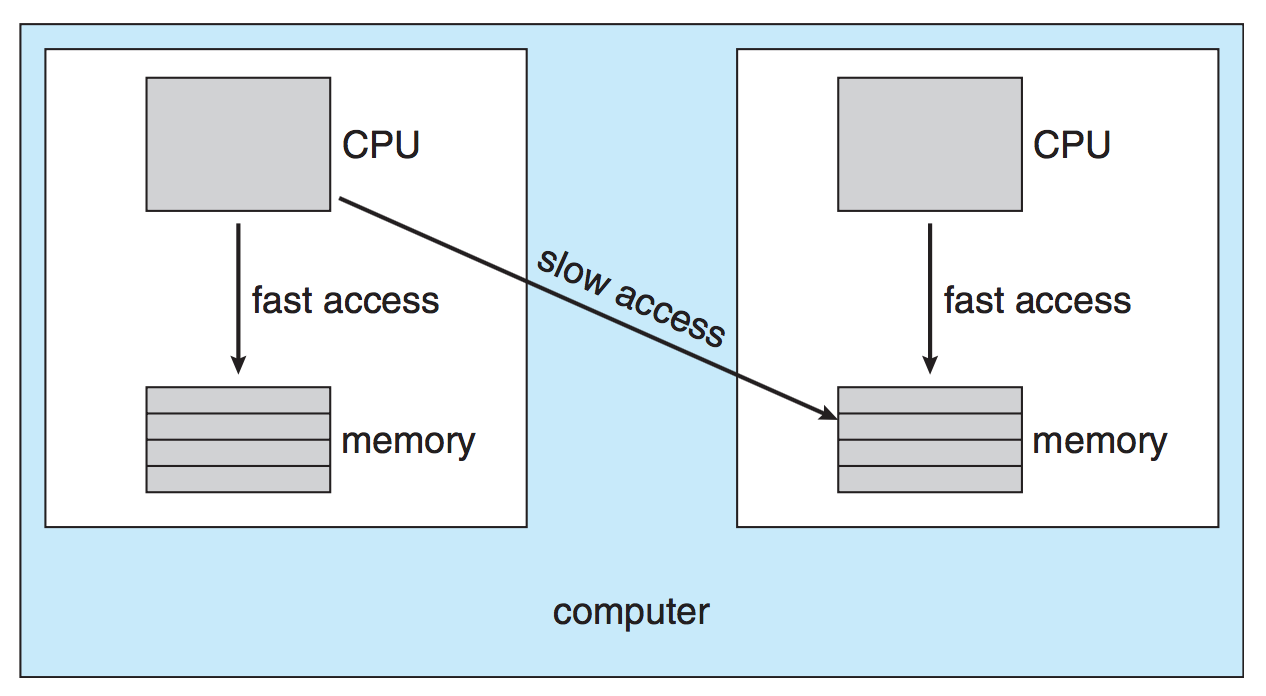
\includegraphics[width=0.5\textwidth]{images/numa.png}\\
	A system with Non-Uniform Memory Access (NUMA) times~\cite{osc}.
\end{center}

If we have this situation, then our choice of processor should be based on where the memory of the process is located. The memory allocation routine should also pay attention to where to allocate memory requests, preferring to keep the program code together in memory. If there is data in one of the other blocks of memory, it does not mean game over, but it means slower execution.

\subsection*{Load Balancing}
It is presumably obvious that if we have 4 processors, it is less than ideal to have one processor at 100\% utilization and 3 processors sitting around doing nothing. We want to keep the workload balanced between all the different systems. The process for this is \textit{load balancing}.

Load balancing is typically necessary only where each processor has its own private queue of processes to run (the ``grocery store queue'' model); if there is a common ready queue (the ``bank queue'' model) then load balancing will tend to happen all on its own, as a processor with nothing to do will simply take the next process from the queue. But in most of the modern operating systems we are familiar with, each processor does have a private queue, so we need to do load balancing~\cite{osc}.

There are two, non-exclusive approaches to redistributing the load: \textit{push} and \textit{pull} migration. It is called migration because a process migrates from one processor to another (it moves homes). If there is push migration, a task periodically checks how busy each processor is and then moves processes around to balance things out (to within some tolerance). Pull migration is when a processor with nothing to do ``steals'' a process from the queue of a busy processor. The Linux and FreeBSD schedulers, for example, use both~\cite{osc}.

Load balancing, as you can imagine, sometimes conflicts with processor affinity. If a process has a hard affinity for a processor, it cannot be migrated from one processor to another. If there is a soft affinity, it can be moved, but it is presumably not our first choice and we will move that process only if we have no other option. Even then, we might consider what to do: should we always move a process despite the fact that it means a whole bunch of cache misses? Should we never do so and leave processors idle? Perhaps the best thing to do is to put a certain ``penalty'' on moving and only move a process from one queue to another if it would be worthwhile (i.e. the imbalance is sufficiently large).

\subsection*{Multicore Processors}
Before the early 2000s, the only way to get multiple processors in the system was to have multiple physical chips. But if you open up your laptop you are likely to find one physical chip. What gives? \textit{Multicore processors}. As far as the operating system is concerned, a quad-core chip is made of four logical processors, but it's all in one package and this can be faster and more convenient.

When a processor issues a memory read or write that is a cache miss (so the read has to go to memory), the CPU core can spend a lot of time (perhaps as much as 50\%) of its time waiting for that read to take place. We might refer to periods of time where there is computation as a compute cycle, and time spent waiting for memory as a \textit{memory stall}. These tend to alternate, though the length of time for each will vary significantly. It's all a question of how often memory is accessed and how many cache misses there are. See the diagram below:

\begin{center}
	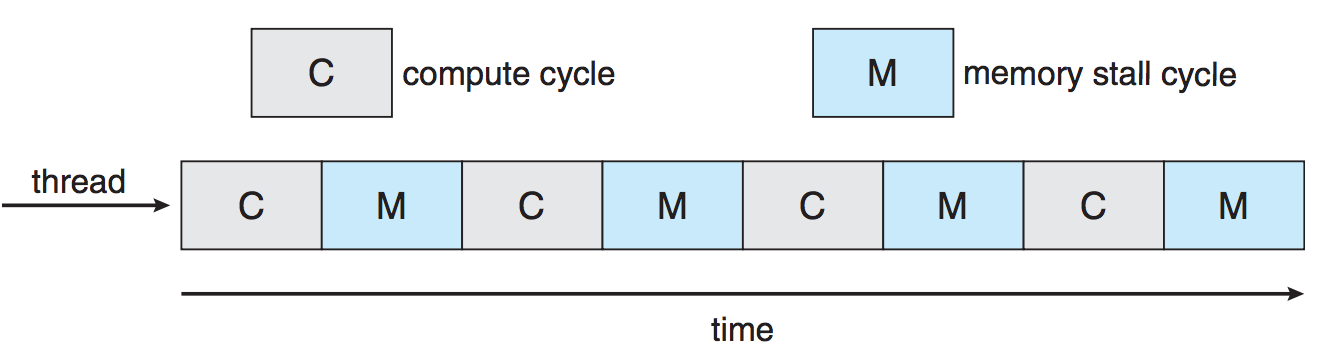
\includegraphics[width=0.7\textwidth]{images/memory-stall.png}\\
	Alternating compute and memory stall cycles~\cite{osc}.
\end{center}

During a memory stall, the processor core may have nothing to do. As you might learn about if you take a course in processor design or programming for performance, you can sometimes move instructions around so that the memory read goes out ``early'' and a few other instructions can be executed in the meantime. 

To offset this problem, the solution was originally called \textit{hyperthreading}: two threads are assigned to each core; if one thread does a memory access or stalls, the code can switch to another thread with a limited penalty. The first CPU I had with hyperthreading was a Pentium IV (it was 2003), and it had one physical core but it would seemingly work on two threads at a time. See below:

\begin{center}
	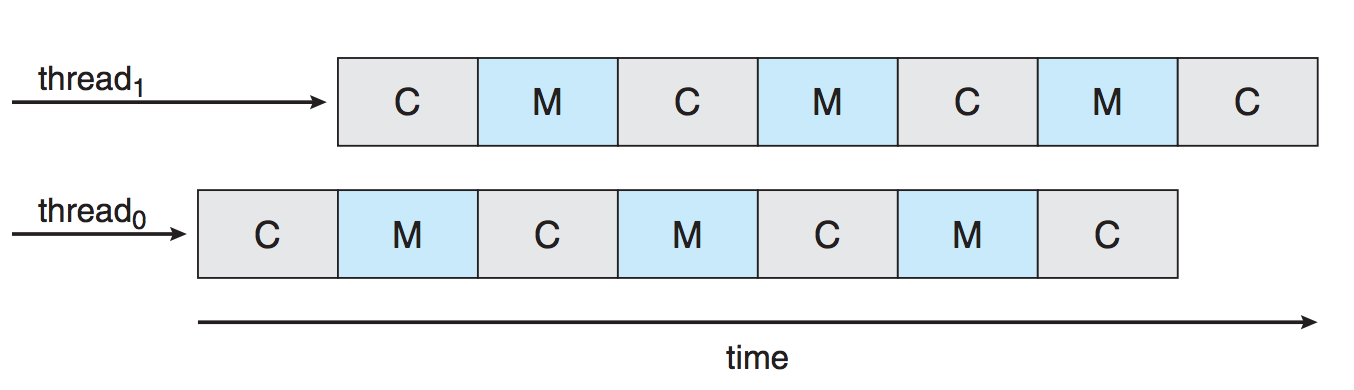
\includegraphics[width=0.7\textwidth]{images/hyperthreading.png}\\
	Hyper threading in a single CPU core~\cite{osc}.
\end{center}

If we have coarse-grained multithreading, a thread will execute for a while and when there is a memory stall (or some other reason why a process gets blocked) then the processor will swap to another thread or process, flushing the instruction pipeline. That is expensive. If we have fine-grained multithreading, it looks more like the diagram above where we have alternation between two threads that are in the pipeline at the same time. The cost of switching between these two threads is small~\cite{osc}.

So now we have two different levels of scheduling: assigning a process or thread to a processor (the job of the operating system) and deciding when to swap between the two threads in the core (typically the job of the hardware). 

\section*{Real-Time Scheduling}
Long ago, this course was ``real time operating systems'' and there was a small amount of emphasis given to the subject of real time systems. A tiny bit of this is preserved in this section about real-time scheduling, that is to say, scheduling for real-time systems. But what is a real-time system? It is one that is supposed to respond to events within a certain amount of real (wall-clock) time. There are deadlines, and there are consequences for missing deadlines. Furthermore, fast is not as important as predictable. If real time systems are of interest to you, you may wish to take some of the later embedded systems courses, or the famous CS trains course\footnote{Abandon sanity, all ye who enter here.}.

As a general note, most of the operating systems you are familiar with (standard Desktop/Server Linux, Mac OS, Windows) are not very suitable to real time systems. They make few guarantees, if any, about service. When there are consequences for missing deadlines, this kind of thing matters. This was, as we already discussed, a reason why Java is not a very good choice for a real-time system: the garbage collector runs whenever it pleases and can ``stop the world'' (halt all execution) until that is finished. And how long is that going to take? Nobody knows.

In Windows you can set a high priority (e.g. level 31) to a process and it calls the priority ``Realtime'', but please don't be fooled: this does not mean it guarantees it will make a particular deadline.

\subsection*{Timeline Scheduling}
If a process or task recurs at regular intervals, it is \textit{periodic} -- repeats at a fixed period. Periodic tasks are very common: check a sensor, decode and display a frame of video to a screen, keep the wifi connection alive, etc.

Consider a periodic task to have two attributes: $\tau_{k}$, the period (how often the task takes) and $c_{k}$, the computation time (how long, in the worst case, the task might execute). In real-time systems we are usually pessimists and care almost exclusively about the worst case scenario. We can calculate the processor utilization of period tasks according to the following formula, to get the long-term average of processor utilization $U$~\cite{mte241}:

\begin{center}
$U = \sum\limits_{k=1}^n\dfrac{c_{k}}{\tau_{k}}$
\end{center}

If $U > 1$, it means the system is overloaded: there are too many period tasks and we cannot guarantee that the system can execute all tasks and meet the deadlines. Otherwise, we will be able to devise a schedule of some sort that makes it all work.

If the only tasks in the system are periodic ones, then we can create a fixed schedule for them. This is what the university administrators do when they create the schedule of classes for a given term. Every Monday, for example, from 13:30-14:50, course ECE~254 (a ``process'', if you will) takes place in classroom EIT~1015 (a resource). There is no way to have two classes in the same lecture hall at the same time, so if there are more requests for room reservations than rooms and time slots available, it means some requests cannot be accommodated.

A world in which all the tasks are periodic and behave nicely is, well, a very orderly world (and that has its appeal). Unfortunately, the real world is not so accommodating most of the time. So we will need to deal with tasks that are not periodic, which we can categorize as \textit{aperiodic} or \textit{sporadic}.


\bibliographystyle{alpha}
\bibliography{254}


\end{document}